\documentclass{article}

\usepackage{amsmath}
\usepackage{amssymb}
\usepackage{amsthm}
\usepackage[hidelinks]{hyperref}
\usepackage{xcolor}
\usepackage{graphicx}

\usepackage{geometry}
 \geometry{
 a4paper,
 total={170mm,257mm},
 left=20mm,
 top=20mm,
 }
\usepackage{blindtext}
\usepackage{lastpage}
\usepackage{fancyhdr}
\pagestyle{fancy}
\fancyhf{} 
\fancyfoot[R]{Page \thepage}

\newtheorem{definition}{Definition}
\newtheorem{theorem}{Theorem}
\newtheorem{lemma}{Lemma}
\newtheorem{proposition}{Proposition}
\newtheorem{example}{Example}
\newtheorem{corollary}{Corollary}

\begin{document}

Basic properties of complex numbers $z=x+iy$ are not mentioned here. Based on the definition of the absolute value (norm) of the complex number: $|z|=(x^2+y^2)^{1/2}$, two interesting properties are listed below:

\begin{enumerate}
\item
Triangle inequality: $|z_1+z_2|\leq|z_1|+|z_2|$

\item
$|z_1-z_2|\geq||z_1|-|z_2||$
\end{enumerate}
The first property can be verified by thinking of the complex number as a vector in $\mathbb{R}^2$ with the real part and complex part being respectively the first and second coordinates. The second property can be proved as follows:

\begin{proof}
If we can show both $|z_1-z_2|\geq|z_1|-|z_2|$ and $|z_1-z_2|\geq|z_2|-|z_1|$, then we are done. From the triangle inequality, we have:

\begin{equation*}
\begin{aligned}
&|z_1|=|z_2+z_1-z_2|\leq|z_2|+|z_1-z_2|\Rightarrow |z_1|-|z_2|\leq|z_1-z_2|\\
&|z_2|=|z_1+z_2-z_1|\leq|z_1|+|z_2-z_1|\Rightarrow |z_2|-|z_1|\leq|z_2-z_1|=|z_1-z_2|
\end{aligned}
\end{equation*}
\end{proof}

Roughly speaking, for a complex function $f:\mathbb{C}\rightarrow\mathbb{C}$, if $\frac{f(z+h)-f(z)}{h}$ converges as $h\rightarrow0$, then we say $f$ is holomorphic. Note that $h$ can go to $0$ from different directions, i.e., from the real axis, the complex axis, or many more. Being a holomorphic function in an open set $\Omega$ enables a lot of miracle to happen, such as:

\begin{enumerate}
\item
Contour integration: for closed paths, the contour integration of $f$ equals 0, independent of the parametrization.

\item
Regularity: $f$ is differentiable infinitely many times, and it has a convergent power series (Taylor series expansion).

\item
Analytic continuation: if $f$ and $g$ agree on a (possibly tiny) open subset of $\Omega$, then they agree on all $\Omega$.
\end{enumerate}

Note that the complex space is complete, which implies that a sequence converges if and only if it is a Cauchy sequence.

We recall several basic properties of a set here.

\begin{definition}\textcolor{red}{(Interior Point)}

For a set $\Omega$, $z\in\Omega$ is called the interior point if there exists $r>0$ such that the disk $D_r(z):={w\in\mathbb{C}:|z-w|<r}$ is contained in $\Omega$.
\end{definition}

\begin{definition}\textcolor{red}{(Open Set)}

A set $\Omega$ is called open if every point in it is an interior point.
\end{definition}

\begin{definition}\textcolor{red}{(Closed Set)}

A set $\Omega$ is called closed if its complement is an open set.
\end{definition}

\begin{definition}\textcolor{red}{(Connected Open Set)}

A open set $\Omega$ is called connected if it is not possible to find two disjoint open set $U_1$ and $U_2$ such that $\Omega=U_1\cup U_2$.
\end{definition}

\begin{definition}\textcolor{red}{(Region)}

A region is an open connected set.
\end{definition}

Now, we properly define the holomorphic here. 

\begin{definition} \label{def:holomorphic} \textcolor{red}{(Holomorphic Function)}

Let $f$ be a complex function on an open set $\Omega$. $f$ is holomorphic at the point $z\in\Omega$ if $\frac{f(z+h)-f(z)}{h}$ converges, as $h$ converges to $0$. Its limited is denoted as $f'(z)$. $f$ is called a holomorphic function if it is holomorphic at every point point in $\Omega$. 
\end{definition}

\begin{example}
$f(z)=z$ is holomorphic because $\frac{f(z+h)-f(z)}{h}=\frac{z+h-z}{h}=1$
\end{example}

\begin{example} \label{ex:non_holomorphic}
$f(z)=\bar{z}$ is not holomorphic because $\frac{f(z+h)-f(z)}{h}=\frac{\bar{z}+\bar{h}-\bar{z}}{h}=\frac{\bar{h}}{h}$. If $h$ is real, then $f'(z)=1$, but if $h$ is imaginary, $f'(z)=-1$.
\end{example}

It is clear from Definition \ref{def:holomorphic} that $f$ is holomorphic at a point $z\in\Omega$ if and only if there exists a complex number $a$ such that 

\begin{equation} \label{holomorphic}
f(z+h)-f(z)-ah=h\psi(h),
\end{equation}
where $\psi$ is a function defined for small $h$ and $\lim_{h\rightarrow0}\psi(h)=0$. \eqref{holomorphic} can be used to show the following properties.

\begin{proposition}
If $f$ and $g$ are holomorphic in $\Omega$, then
\begin{enumerate}
\item
$f+g$ is holomorphic

\item
$fg$ is holomorphic

\item
$(f+g)'=f'+g'$

\item
$(fg)'=f'g+fg'$
\end{enumerate}
\end{proposition}

The notion of complex differentiability differs significantly from the real differentiability. As seen from Example \ref{ex:non_holomorphic}, if we interpret the complex function $f(z)=\bar{z}$ as a real function with two coordinates, then $f(z)=f(x,-y)$, which is differentiable in the real sense. Now, we build the link between real and complex functions through the Cauchy-Riemann equation. 

Suppose $f$ is holomorphic at $z_0=x_0+iy_0$, and let $h=h_1+ih_2$. Consider $f(z)=f(x,y)$. If $h_1=0$, we have

\begin{equation*}
\lim_{h_2\rightarrow0}\frac{f(x_0,y_0+h_2)-f(x_0,y_0)}{ih_2}=\frac{1}{i}\frac{\partial f}{\partial y}.
\end{equation*}
Similarly, if $h_2=0$, we have

\begin{equation*}
\lim_{h_1\rightarrow0}\frac{f(x_0+h_1,y_0)-f(x_0,y_0)}{h_1}=\frac{\partial f}{\partial x}.
\end{equation*}
Since $f$ is holomorphic at $z_0$, we have the first Cauchy-Riemann equation as follows:

\begin{equation} \label{Cauchy_Riemann}
\frac{\partial f}{\partial x}=\frac{1}{i}\frac{\partial f}{\partial y}.
\end{equation}

If we write the holomorphic function as $f(z)=u(x,y)+iv(x,y)$, then we have the following relation:

\begin{equation} \label{Cauchy_Riemann_2}
\begin{aligned}
&\frac{\partial u}{\partial x}=\frac{\partial v}{\partial y}\\
&\frac{\partial v}{\partial x}=-\frac{\partial u}{\partial y}.
\end{aligned}
\end{equation}

We also have the following results from the Cauchy-Riemann equation

\begin{proposition}
If $f$ is holomorphic at $z_0$, then 

\begin{equation}
\frac{\partial f}{\partial\bar{z}}(z_0)=0 \quad \text{and} \quad f'(z_0)=\frac{\partial f}{\partial z}(z_0)=2\frac{\partial u}{\partial z}(z_0)
\end{equation}

\end{proposition}

\begin{proof}
For $z=x+iy$, we know $x=\frac{1}{2}(z+\bar{z})$ and $y=\frac{1}{2i}(z-\bar{z})$. Then, we can define the following two differential operators

\begin{equation*}
\begin{aligned}
&\frac{\partial f}{\partial z}=\frac{\partial f}{\partial x}\frac{\partial x}{\partial z}+\frac{\partial f}{\partial y}\frac{\partial y}{\partial z}=\frac{1}{2}\frac{\partial f}{\partial x}+\frac{1}{2i}\frac{\partial f}{\partial y}\\
&\frac{\partial f}{\partial \bar{z}}=\frac{\partial f}{\partial x}\frac{\partial x}{\partial \bar{z}}+\frac{\partial f}{\partial y}\frac{\partial y}{\partial \bar{z}}=\frac{1}{2}\frac{\partial f}{\partial x}-\frac{1}{2i}\frac{\partial f}{\partial y}.
\end{aligned}
\end{equation*}
From $\eqref{Cauchy_Riemann}$, we have the desired result $\frac{\partial f}{\partial\bar{z}}(z_0)=0$.

For the second result, first observe

\begin{equation*}
\frac{\partial f}{\partial z}(z_0)=\frac{1}{2}\frac{\partial f}{\partial x}(z_0)+\frac{1}{2i}\frac{\partial f}{\partial y}(z_0)=\frac{\partial f}{\partial x}(z_0)
\end{equation*}
Then, using the operator $\frac{\partial}{\partial z}$ defined above, we have
\begin{equation*}
\frac{\partial u}{\partial z}(z_0)=\frac{1}{2}\frac{\partial u}{\partial x}(z_0)+\frac{1}{2i}\frac{\partial u}{\partial y}(z_0)=\frac{1}{2}(\frac{\partial u}{\partial x}(z_0)+i\frac{\partial v}{\partial x}(z_0))=\frac{1}{2}\frac{\partial f}{\partial x}(z_0),
\end{equation*}
which directly leads to the second result.
\end{proof}

So far, we have assumed $f$ to be holomorphic and deduced the relation between its real and imaginary parts. In the next theorem, we show that the converse is also true, which completes the circle. 

\begin{theorem}
Suppose the complex function $f=u(x,y)+iv(x,y)$ is defined on an open set $\Omega$. If $u$ and $v$ are differentiable and satisfy the Cauchy-Riemann equation \eqref{Cauchy_Riemann_2} on $\Omega$, then $f$ is holomorphic on $\Omega$, and $f'(z)=\partial f/\partial z$.
\end{theorem}

\begin{proof}
Since $u$ and $v$ are differentiable, we have 

\begin{equation*}
\begin{aligned}
&u(x+h_1,y+h_2)-u(x,y)=\frac{\partial u}{\partial x}h_1+\frac{\partial u}{\partial y}h_2+|h|\psi_1(h)\\
&v(x+h_1,y+h_2)-v(x,y)=\frac{\partial v}{\partial x}h_1+\frac{\partial v}{\partial y}h_2+|h|\psi_2(h),
\end{aligned}
\end{equation*}
where $\psi_1(h),\psi_2(h)\rightarrow0$ as $|h|\rightarrow0$, and $h=h_1+ih_2$. Using \eqref{Cauchy_Riemann_2}, we have:

\begin{equation*}
\begin{aligned}
f(z+h)-f(z)&=f(x+f_1+iy+ih_2)-f(x+iy)\\
&=u(x+h_1,y+h_2)+iv(x+h_1,y+h_2)-u(x,y)-iv(x,y)\\
&=\frac{\partial u}{\partial x}h_1+\frac{\partial u}{\partial y}h_2+|h|\psi_1(h)+\frac{\partial v}{\partial x}h_1+\frac{\partial v}{\partial y}h_2+|h|\psi_2(h)\\
&=\left(\frac{\partial u}{\partial x}-i\frac{\partial u}{\partial y}\right)(h_1+ih_2)+|h|\psi_1(h)+|h|\psi_2(h),
\end{aligned}
\end{equation*}
which implies

\begin{equation*}
\begin{aligned}
\frac{f(z+h)-f(z)}{h}&=\left(\frac{\partial u}{\partial x}-i\frac{\partial u}{\partial y}\right)+\frac{|h|\psi_1(h)+|h|\psi_2(h)}{h}\\
&\rightarrow\left(\frac{\partial u}{\partial x}-i\frac{\partial u}{\partial y}\right)\\
&=2\frac{\partial u}{\partial z}\\
&=\frac{\partial f}{\partial z}.
\end{aligned}
\end{equation*}
\end{proof}

\begin{definition} \textcolor{red}{(Power Series)}

A power series is an expansion of the form $\sum^\infty_{n=0}a_nz^n$.
\end{definition}

\begin{definition} \textcolor{red}{(Absolute Convergence)}

A power series is said to converge absolutely if $\sum^\infty_{n=0}|a_nz^n|$ converges.
\end{definition}

\begin{definition} \textcolor{red}{(Analytic Function)}

We say that a function is analytic in an open set $\Omega$ if it has a convergent power series expansion in $\Omega$
\end{definition}

We give the following result about the convergence of a power series without proof. 

\begin{theorem} \textcolor{red}{(Convergence of Power Series)}

Given a power series $\sum^\infty_{n=0}a_nz^n$, there exists $0\leq R\leq\infty$ such that:

\begin{enumerate}
\item
If $|z|<R$, the series converges absolutely.

\item
If $|z|>R$, the series diverges.
\end{enumerate}

The radius of convergence $R$ is given by the Hadmard's formula as follows:

\begin{equation}
\frac{1}{R}=\limsup_{n\rightarrow\infty}|a_n|^{1/n}.
\end{equation}
\end{theorem}

Power series provide a very important class of analytic functions that are particularly simple to manipulate, as shown in the following theorem. 

\begin{theorem}
The power series $f(z)=\sum^\infty_{n=0}a_nz^n$ define a holomorphic function in its disk of convergence. The derivative of $f$ is also a power series obtained by differentiating term be term, i.e. $f'(z)=\sum^\infty_{n=0}na_nz^{n-1}$. Additionally, $f'(z)$ has the same radius of convergence. 
\end{theorem}

\begin{proof}
We aim to show the following:

\begin{equation*} 
\lim_{h\rightarrow0}|\frac{f(z+h)-f(z)}{h}-g(z)|=0,
\end{equation*}
where $g(z):=\sum^\infty_{n=0}na_nz^{n-1}$. Only main steps are shown here. The intuition is to separate the infinite sum of $f$ into a finite sum and a tail part, because the finite sum is essentially a polynomial, and its derivative is obtained by differentiating term by term. 

Define the following terms

\begin{equation*}
\begin{aligned}
&S_N:=\sum^N_{n=0}a_nz^n\\
&E_N:=\sum^\infty_{n=N+1}a_nz^n\\
&S'_N:=\sum^N_{n=0}na_nz^{n-1}.
\end{aligned}
\end{equation*}
Then, 
\begin{equation*}
\begin{aligned}
\lim_{h\rightarrow0}|\frac{f(z+h)-f(z)}{h}-g(z)|&=\lim_{h\rightarrow0}|\frac{S_N(z+h)-S_N(z)}{h}+\frac{E_N(z+h)-E_N(z)}{h}+S'_N-S'_N-g(z)|\\
&\leq \lim_{h\rightarrow0}\{|\frac{S_N(z+h)-S_N(z)}{h}-S'_N|+|\frac{E_N(z+h)-E_N(z)}{h}|+|S'_N-g(z)|\}.
\end{aligned}
\end{equation*}
The first term vanishes because polynomials are differentiable, and the derivate is obtained term by term. The last term vanishes because $\lim_{N\rightarrow\infty}S'_N=g(z)$. The second term also vanishes based on the following two facts

\begin{enumerate}
\item
$a^n-b^n=(a-b)(a^{n-1}+a^{n-2}b+a^{n-3}b^2+...+ab^{n-1}+b^{n-1})$

\item
$\sum^\infty_{n=N+1}na_nz^{n-1}$ is the tail of a convergence sequence and thus vanishes.
\end{enumerate}

Finally, $f'$ and $f$ have the same radius of convergence from the Hadmard's formula and the fact that $\lim_{n\rightarrow\infty}n^{1/n}=1$.

\end{proof}

Now, we change our focus to integration of complex functions along curves. First, we give several definitions

\begin{definition} \textcolor{red}{(Primitive)}

A primitive of $f$ on $\Omega$ is a function $F$ that is holomorphic on $\Omega$ and such that $F'(z)=f(z)$ for all $z\in\Omega$.
\end{definition}

\begin{definition} \textcolor{red}{(Parametrized Curve)}

A parametrized curve is a function $z(t)$ which maps a closed interval $[a,b]\subset\mathbb{R}$ to the complex plane.
\end{definition}

The integral of $f$ along a curve $\gamma$ is then defined as

\begin{equation*}
\int_\gamma f(z)dz:=\int_a^b f(z(t))z'(t)dt.
\end{equation*}

In order for this definition to make sense, one can also show that it is independent of the choice of the parametrization. By definition, the length of the smooth curve $\gamma$ is 

\begin{equation*}
\text{length($\gamma$)}=\int_a^b |z'(t)|dt.
\end{equation*}

We may then develop an useful bound, called the M-L bound, for the integration over curves:

\begin{equation} \label{M_L_bound}
\begin{aligned}
|\int_\gamma f(z)dz| = |\int^b_a f(z(t))z'(t)dt|\leq\int^b_a |f(z(t))z'(t)|dt\leq\sup_{z\in\gamma}|f(z(t))|\int^b_a |z'(t)|dt=\sup_{z\in\gamma}|f(z(t))|\text{length($\gamma$)}.
\end{aligned}
\end{equation}

Assuming $f$ has a primitive, many useful results arise.

\begin{theorem} \label{thm_int_end_points}
If $f$ has a primitive $F$ in $\Omega$, and $\gamma$ is a curve in $\Omega$ that has end points $w_1$ and $w_2$, then 

\begin{equation*}
\int_\gamma f(z)dz=F(w_1)-F(w_2)
\end{equation*}
\end{theorem}

\begin{proof}
The proof is quite straightforward. By definition,

\begin{equation*}
\begin{aligned}
\int_\gamma f(z)dz=\int^b_a f(z(t))z'(t)dt=\int^b_aF'(z(t))z'(t)dt=\int^b_a\frac{d}{dt}F(z(t))dt=F(z(b))-F(z(a))=F(w_1)-F(w_2).
\end{aligned}
\end{equation*}
\end{proof}

Next, we state several corollaries from this theorem, the proofs of which are very simple, so they are omitted. 

\begin{corollary} \label{cor:primitive_int_zero}
If $\gamma$ is a closed curve in an open set $\Omega$, and $f$ has a primitive in $\Omega$, then

\begin{equation} \label{primitive_int_zero}
\int_\gamma f(z)dz=0.
\end{equation}
\end{corollary}

\begin{corollary}
If $f$ is holomorphic in a region $\Omega$, and $f'=0$, then $f$ is constant. 
\end{corollary}

\begin{corollary}
If $f$ has a primitive in $\Omega$, then the integral does not depend on the choice of the path. 
\end{corollary}

Corollary \ref{cor:primitive_int_zero} gives us one direction, and we would like to show the converse, namely if we know that \eqref{primitive_int_zero} for some types of curves $\gamma$, then a primitive for $f$ exists. We start with the Goursat's theorem.

\begin{theorem} \textcolor{red}{(Goursat)}
If $f$ is holomorphic in an open set $\Omega$, and $T\subset\Omega$ is a triangle whose interior is also contained in $\Omega$, then

\begin{equation*}
\int_T f(z)dz=0.
\end{equation*}

\end{theorem}

\begin{figure}
\centering
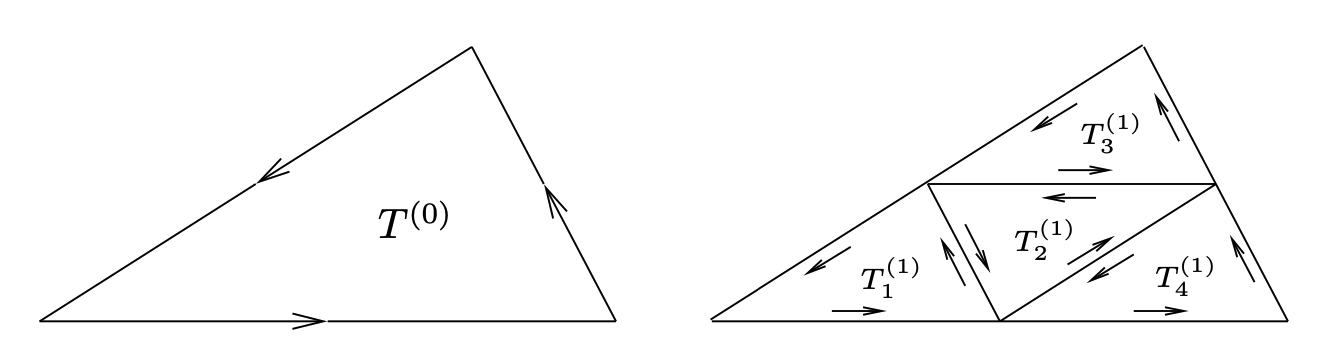
\includegraphics[scale=0.3]{Goursat.png} \\
\caption{Bisecting triangle in the proof of Goursat's Theorem.} 
\label{fig:goursat}
\end{figure}

\begin{proof}
The proof is based on this brilliant idea of recursively bisecting the triangle, as shown in Fig. \ref{fig:goursat}. The subscript counts the number of triangles, and the superscript represents the iteration. Only main steps of the proof are shown here. 

In the first iteration, we have:

\begin{equation*}
\begin{aligned}
\int_{T^{(0)}} f(z)dz&=\int_{T_1^{(1)}} f(z)dz+\int_{T_1^{(2)}} f(z)dz+\int_{T_1^{(3)}} f(z)dz+\int_{T_1^{(4)}} f(z)dz\\
&\leq4\int_{T_j^{(1)}} f(z)dz,
\end{aligned}
\end{equation*}
for some $j$ that gives the maximum integral value, and we name this triangle $T^{(1)}$. Repeating this process for $k$ times, we obtain

\begin{equation*}
\begin{aligned}
|\int_{T^{(0)}} f(z)dz|\leq4^k|\int_{T^{(k)}} f(z)dz|.
\end{aligned}
\end{equation*}

We may prove that there is a unique $z_0$ in every triangle $\{T^{(n)}\}_{n=1,...,k}$. Since $f$ is holomorphic at $z_0$, we have

\begin{equation*}
f(z)=f(z_0)+f'(z_0)(z-z_0)+\psi(z-z_0)(z-z_0),
\end{equation*}
where $\psi(z-z_0)\rightarrow0$ as $z\rightarrow z_0$. The constant $f(z_0)$ and $f'(z_0)(z-z_0)$ has primitives, so they have zero integral value over the closed curve $T^{(k)}$. Finally, $|\int_{T^{(k)}} f(z)dz|$ can be bounded by the M-L bound \eqref{M_L_bound}  and the following two facts:

\begin{enumerate}
\item
perimeter of $T^{(k)}$=$\frac{1}{2^k}\times$ perimeter of $T^{(0)}$

\item
diameter of $T^{(k)}$=$\frac{1}{2^k}\times$ diameter of $T^{(0)}$
\end{enumerate}

Then, it is straightforward to show $\lim_{k\rightarrow\infty}4^k|\int_{T^{(k)}} f(z)dz|=0$, which completes the proof. 

\end{proof}

Next, we prove the existence of primitive in a disk as a consequence of Goursat's Theorem. 

\begin{theorem} \textcolor{red}{(Local Existence of Primitives)}

A holomorphic function in an open disk has a primitive in that disk.
\end{theorem}

\begin{figure}
\centering
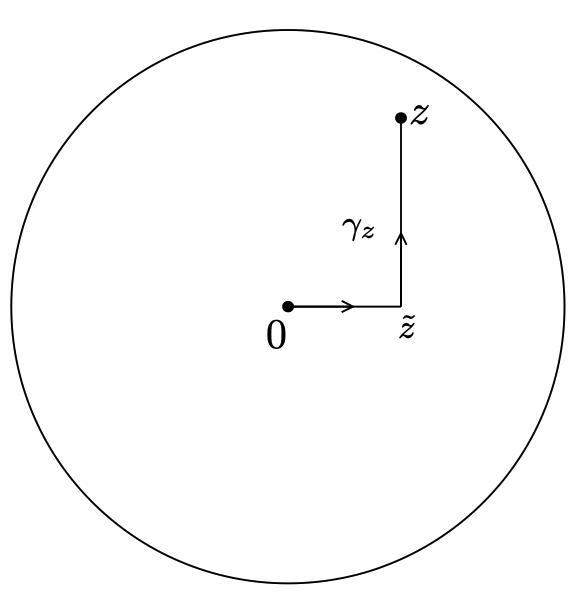
\includegraphics[scale=0.3]{local_primitive_1.png} \\
\caption{Open disk with the choice of curve $\gamma_z$} 
\label{fig:local_primitive_1}
\end{figure}

\begin{figure}
\centering
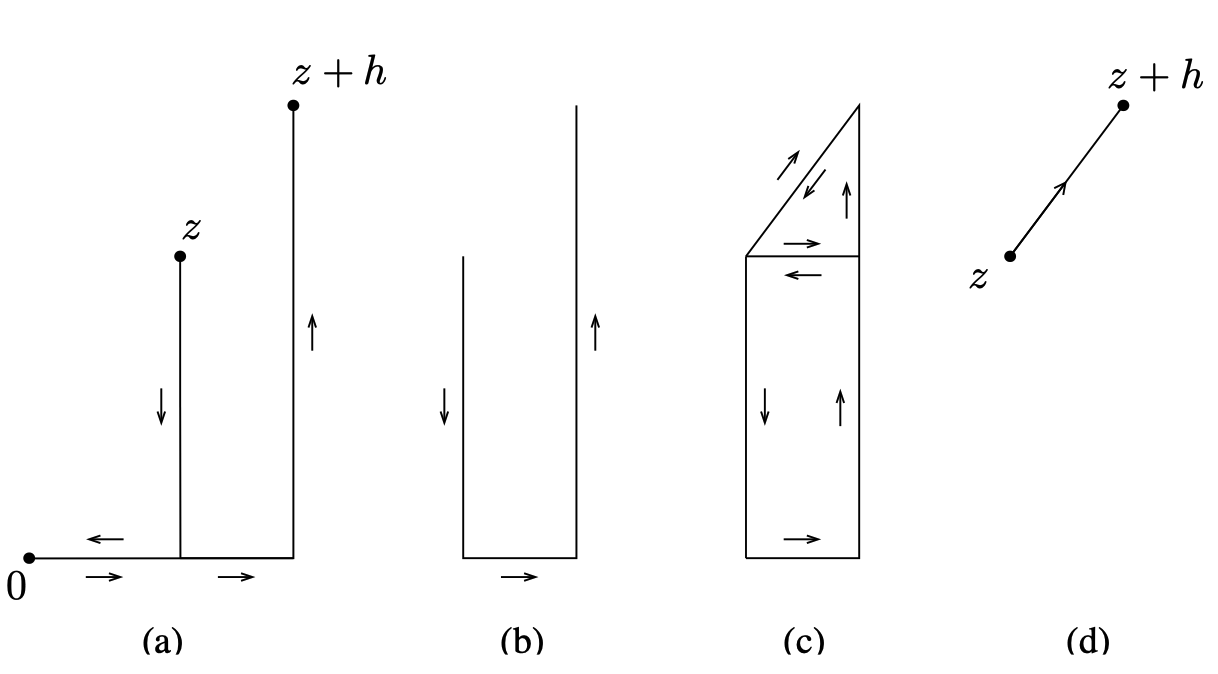
\includegraphics[scale=0.3]{local_primitive_2.png} \\
\caption{Relation between $\gamma_z$ and $\gamma_{z+h}$.} 
\label{fig:local_primitive_2}
\end{figure}

\begin{proof}
We only show main steps. Consider the open disk $D$ centered at the origin, and choose a point $z\in D$ at random. Constructing the curve $\gamma_z$ as shown in Fig \ref{fig:local_primitive_1}. Define

\begin{equation*}
F(z):=\int_{\gamma_z}f(w)dw.
\end{equation*}
We claim that $F(z)$ is holomorphic in the open disk $D$ and $F'(z)=f(z)$, which means that $F$ is the primitive of $f$ in $D$. Now choose another point $z+h\in D$. Following the steps shown in Fig \ref{fig:local_primitive_2}, which uses the Goursat's Theorem, we have

\begin{equation*}
F(z+h)-F(z)=\int_{\gamma_{z+h}}f(w)dw-\int_{\gamma_{z}}f(w)dw=\int_\eta f(w)dw,
\end{equation*}
where $\eta$ is the curve shown in Fig. \ref{fig:local_primitive_2}(d). Since $f$ is holomorphic in $D$, it is continuous at $w$. Then, $f(w)=f(z)+\psi(w),$ where $\psi(w)\rightarrow0$ as $z\rightarrow w$. With the fact that $f(z)$ has a primitive and Theorem \ref{thm_int_end_points}, we have

\begin{equation*}
\lim_{h\rightarrow0}\frac{F(z+h)-F(z)}{h}=f(z),
\end{equation*}
which completes the proof.
\end{proof}

This theorem says that locally, every holomorphic function has a primitive. Now, we can use the previous result to get 

\begin{theorem} \textcolor{red}{(Cauchy's Theorem for a Disk)}

If $f$ is a holomorphic function in a disk, then 

\begin{equation}
\int_\gamma f(z)dz=0,
\end{equation}
for every closed curve $\gamma$ in that disk.

\end{theorem}

\begin{proof}
Since $f$ is a holomorphic function in a disk, by previous result, $f$ has a primitive in that disk. Then, by Corollary \ref{cor:primitive_int_zero}, we have the desired result.
\end{proof}

\begin{corollary}
If $f$ is holomorphic in an open set that contains a circle $C$ and its interior, then

\begin{equation*}
\int_C f(w)dw=0.
\end{equation*}
\end{corollary}

\begin{proof}
We can slightly enlarge the disk with boundary circle $C$ such that $f$ is still holomorphic in it. Then, we can apply Cauchy's theorem to conclude the proof. 
\end{proof}






























\end{document}